\documentclass[12pt, titlepage]{article}

\usepackage{graphicx}
\graphicspath{ {./images/} }
\usepackage{booktabs}
\usepackage{tabularx}
\usepackage{float}
\usepackage{hyperref}
\hypersetup{
    colorlinks,
    citecolor=black,
    filecolor=black,
    linkcolor=red,
    urlcolor=blue
}
\usepackage[round]{natbib}

\title{SE 3XA3: Software Requirements Specification\\Euneva}

\author{Team 9, Euneva
		\\ Mehta, Jash - mehtaj8
		\\ Sharma, Aditya - shara24
		\\ Ren, Zackary - renx11
}

\date{\today}
\begin{document}

\maketitle

\pagenumbering{roman}
\tableofcontents
\listoftables
\listoffigures

\begin{table}[bp]
\caption{\bf Revision History}
\begin{tabularx}{\textwidth}{p{3cm}p{2cm}X}
\toprule {\bf Date} & {\bf Version} & {\bf Notes}\\
\midrule
12/02/2021 & 1.0 & Initial version of Requirements Specification Document\\
\bottomrule
\end{tabularx}
\end{table}

\newpage

\pagenumbering{arabic}

\section{Project Drivers}

\subsection{The Purpose of the Project}

Students may be managing five, six or even seven courses in one semester in addition to any extracurricular commitments they may have. Each course has an array of quizzes and assignments that students can easily lose track of due to the lack of consolidated information. The purpose of this project is to re-implement an existing To-Do list to allow students a way of accessing important dates and deadlines for courses on McMaster’s University portal, Avenue. Balancing work, school and mental health is challenging, especially for younger individuals like students. Alleviating some of the stress from academics helps students avoid mental health issues and live a healthy lifestyle. 

\subsection{The Stakeholders}

\subsubsection{The Client}

The clients of this product are the teaching staff of Software Engineering 3XA3 course that will be actively involved in the pre-development and development of the project. The teaching staff will be involved in the implementation decisions of the product, as well as determining if the project was successfully completed.

\subsubsection{The Customers}

The customers of this product include students and professors attending/teaching at McMaster University. Students gain the ability to collate all assignments across all Avenue linked courses, as well as the ability to allow a better visual representation of upcoming dates and deadlines. Professors can use this product as a way to track student progress, as well as see if sufficient time has been allocated to each project and/or assignment.

\subsubsection{Other Stakeholders}

Other stakeholders of this product include McMaster’s Academic Success Centre, Brightspace (A2L Software), and Group-9 team members. The Academic Success Centre gains the ability to teach time management and productivity tips. Brightspace, the Avenue to Learn software, gains from this product as it compliments the software they have developed.

\subsection{Mandated Constraints}

\subsubsection{Product Constraints}

In order to use the product, users will require an internet connection and a smartphone with either iOS or Android operating systems. Users will not need to remain connected to the internet once the data from Avenue has been collected, but will need to connect to the internet to allow for additional dates and deadlines to be added.

\subsubsection{User Constraints}

Users of this product must have valid login information for Avenue to Learn to allow the product to access the dates and deadlines for each course.

\subsubsection{Time Constraints}

The time frame given to complete this project and deploy the product is 3 months. This limits the amount of features and compromises product quality on the initial release of the software.

\subsubsection{Budget Constraints}

The use of money in the development of this project is not permitted, this may hinder the user experience as well as the amount of features developed.

\subsection{Naming Conventions and Terminology}

\begin{enumerate}
\item \textbf{UI} - User Interface
\item \textbf{UX} - User Experience
\item \textbf{To-Do} - Typical naming convention for a planner
\end{enumerate}

\subsection{Relevant Facts and Assumptions}

\subsubsection{Facts}

\begin{enumerate}
\item The existing application has 1140 lines of code.
\item The existing application does not have web scraping functionality.
\item The existing UI contains the fundamentals of a To-Do list application, but needs additional features to fit our products usage.
\end{enumerate}

\subsubsection{Assumptions}

\begin{enumerate}
\item The application will be operated in an environment with a working internet connection for the initial setup, as well as for updating to-do items.
\item Users using the application for the intended purpose should have valid login credentials for Avenue to Learn.
\item Users are individuals currently attending or employed by McMaster University.
\end{enumerate}

User characteristics should go under assumptions.

\section{Functional Requirements}

\subsection{The Scope of the Work and the Product}

The software product being developed in this document is a To-Do list linked to Avenue to Learn. The To-Do List will allow users with the correct credentials to extract dates and deadlines for assignments and upcoming tests from Avenue to Learn.\\

\noindent The goal of this software system is to provide the user, which in this case, students who attend McMaster University, with a way of organizing tasks, dates, and deadlines in a clearer manner.\\

\noindent The objective that this software system aims to achieve is to provide the user with ease of access to important information that they would require from each course, in an organized but visually appealing manner.\\

\noindent The benefits of this software system is directly linked to student time management, and ease of access to important organized information. Providing the students with an easy way of accessing dates and deadlines relevant to their courses, would allow them to manage their time more efficiently. \\

\noindent \textbf{Deliverables:}
\begin{itemize}
\item Requirements Documentation
\item Functioning Software
\end{itemize}

\noindent \textbf{Deadlines:}
\begin{itemize}
\item Requirements Document Rev 0 - 2021/02/12
\item Proof of Concept Demonstration - 2021/02/22
\item Test Plan Rev 0 - 2021/03/05
\item Design Documentation - 2021/03/18
\item Revision 0 Demonstration - 2021/03/22
\item Final Demonstration (Rev 1) - 2021/04/05
\item Final Documentation (Rev 1) - 2021/04/12 
\end{itemize}

\subsubsection{The Context of the Work}

\begin{figure}[H]
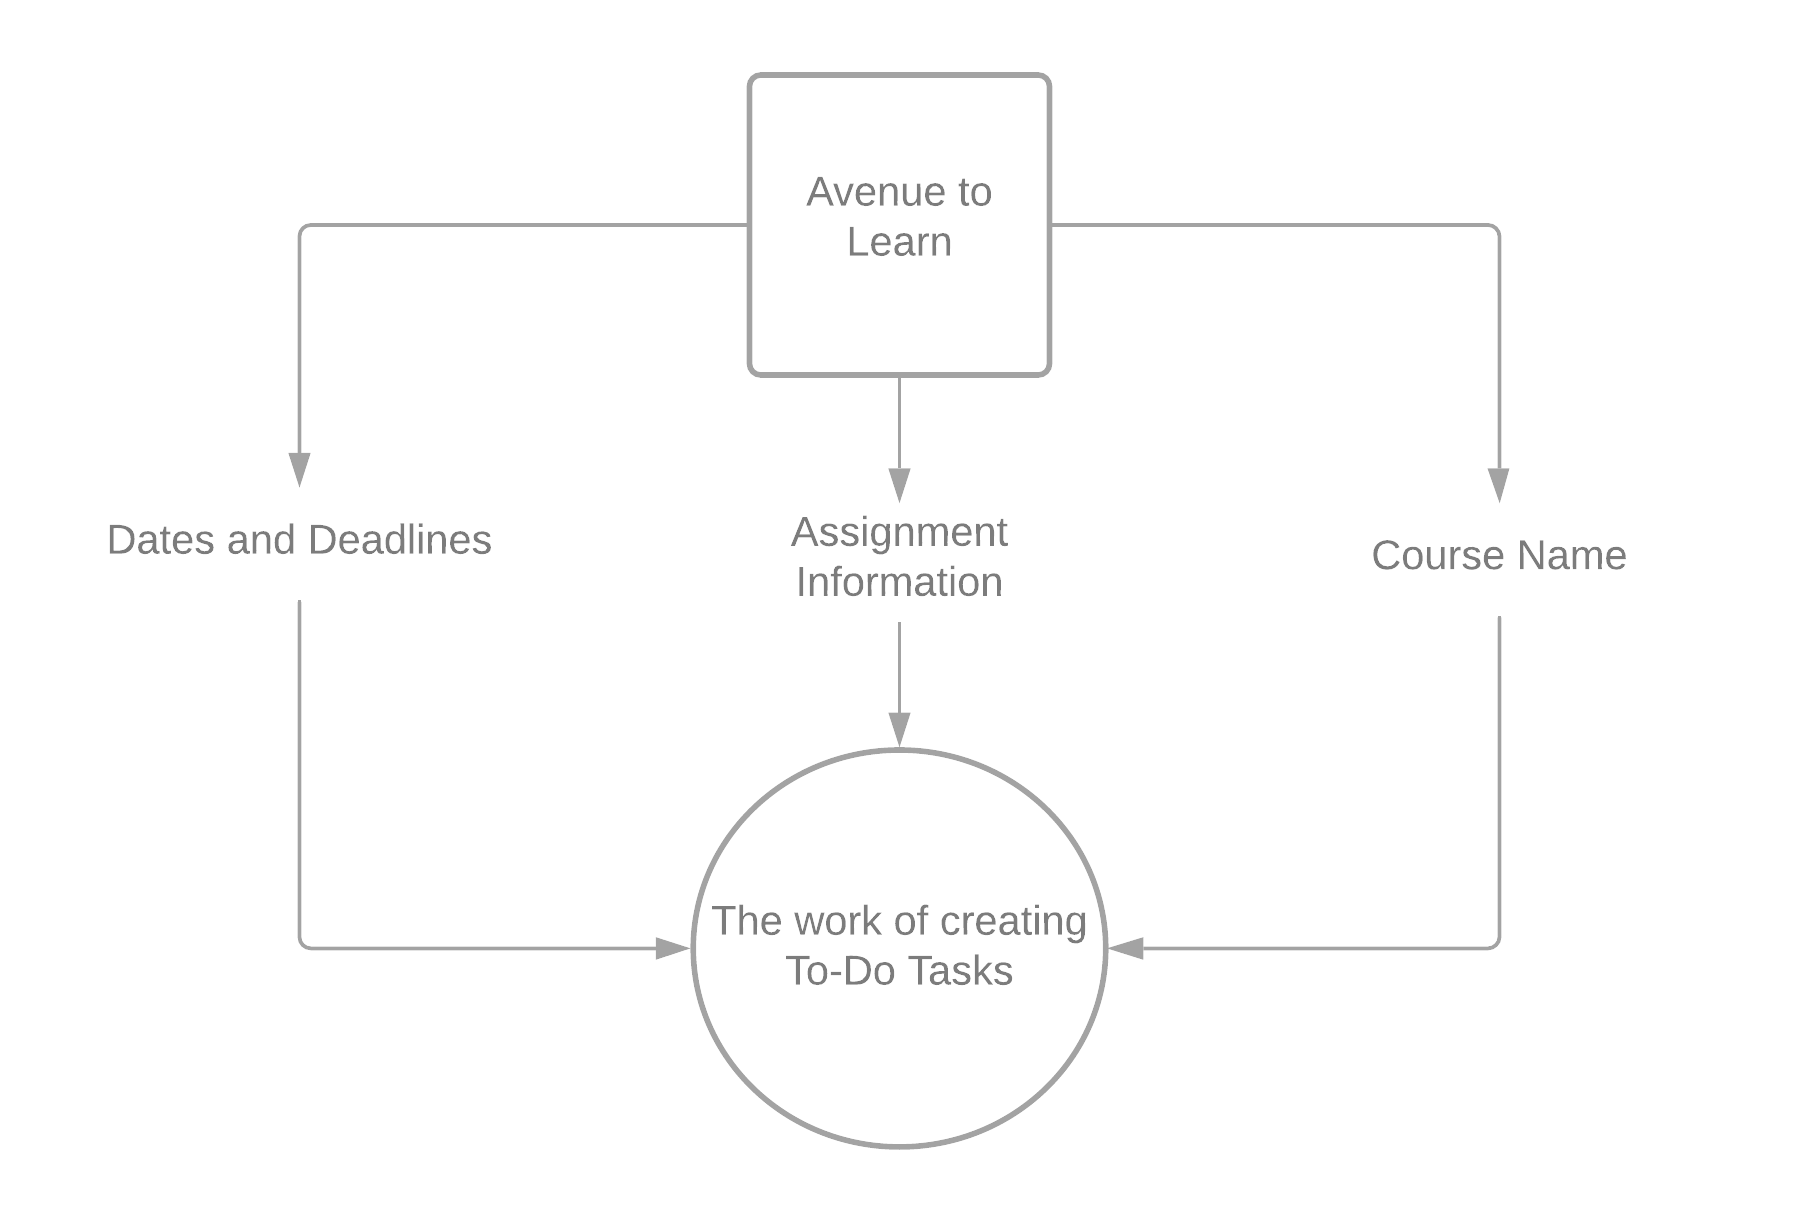
\includegraphics[scale=0.2]{Context_Of_Work}
\caption{Context of Work for Euneva}
\end{figure}

\subsubsection{Work Partitioning}

\begin{table}[H]
\caption{Work Partitioning Part I.}
\begin{center}
\begin{tabular}{ |m{4em}|m{8em}|m{10em}|m{10em}| } 
 \hline
 Event Number & Event Name & Input & Output \\ 
 \hline
 1 & Gather Dates and Deadlines & Avenue to Learn Website & Dates and Deadlines available to use in to-do list \\
 \hline
 2 & Gather Assignment Information & Avenue to Learn Website & Assignment Information available to use with corresponding dates and deadlines\\ 
 \hline
 3 & Gather Course Names & Avenue to Learn Website & Course Names available to use with corresponding dates and deadlines.\\
 \hline 
\end{tabular}
\end{center}
\label{wp1}
\end{table}

\begin{table}[H]
\caption {Work Partitioning Part II.}
\begin{center}
\begin{tabular}{ |m{4em}|m{28em}| } 
 \hline
 Event Number & Summary of Event \\ 
 \hline
 1 & The dates and deadlines for a particular student are found in their account on Avenue to Learn. This allows the usage of dates for our implementation. \\
 \hline
 2 & The Assignment Information collected will be used to attach corresponding dates to allow a more organized list of items.\\ 
 \hline
 3 & The Course names are required for each date and deadline gathered for the same student. This allows for dates to be attached to a name. \\
 \hline 
\end{tabular}
\end{center}
\label{wp2}
\end{table}

\subsubsection{Individual Product Use Cases}

\begin{table}[H]
\caption{Use Cases.}
\begin{center}
\begin{tabular}{ |m{4em}|m{18em}|m{8em}|} 
 \hline
 Actor & Actor’s Goals & Use Case Name \\ 
 \hline
 Student & User links Avenue to Learn account with application. & Login (UC1) \\
 \hline
 Student & User selects courses to be added to the To-Do list. & Select (UC2) \\ 
 \hline
 Student & User edits information of added items from Avenue. & Edit (UC3) \\
 \hline 
 Student & User changes dates of added items. & Edit (UC3) \\
 \hline 
 Student & User deletes items from To-Do list. & Delete (UC4) \\
 \hline 
 Student & User changes state of added To-Do item. & Edit (UC3) \\
 \hline 
\end{tabular}
\end{center}
\label{uc}
\end{table}

\begin{table}[H]
\caption{Use Cases Description.}
\begin{center}
\begin{tabular}{ |m{4em}|m{26em}| } 
 \hline
 Use Case & Description \\ 
 \hline
 Login (UC1) & The user intends to provide login credentials to access Avenue to Learn \\
 \hline
 Select (UC2) & The user intends to select the preferred courses to add to the To-Do list \\ 
 \hline
 Edit (UC3) & The user intends to edit fields in each To-Do item.\\
 \hline 
 Delete (UC4) & The user intends to delete the selected To-Do item from the list.\\
 \hline
\end{tabular}
\end{center}
\label{ucd}
\end{table}

\subsection{Functional Requirements}

FR1. The user interface must include a button for the user to login to Avenue to Learn.
	\textbf{Fit Criterion:} The login button will be displayed on the top right corner of the screen to 
	allow ease of access to login to Avenue to Learn.\\

\noindent FR2. The user interface must include an add task button.
	\textbf{Fit Criterion:} The button will be displayed at the bottom right corner of the screen to 
allow ease of access to add a task\\

\noindent FR3. The user interface must display the date selected.
	\textbf{Fit Criterion:} The date will be displayed on the top left corner of the screen to allow the 
user to view what date the current To-Do Items are located on.\\

\noindent FR4. The user interface must include a date selection at the top of the screen.
	\textbf{Fit Criterion:} The date selection will be displayed under the selected date to allow users 
to select a specific date.\\

\noindent FR5. The user interface must include a way to go to the today date.
	\textbf{Fit Criterion:} The displayed selected date on the top left corner must be a button, when 
pressed sets the date to today.\\

\noindent FR6. The user interface must display a dialog screen after the add task button is pressed.
	\textbf{Fit Criterion:} The displayed dialog should include “Task Name”, “Date”, “Time”, and a 
“Confirm” button to allow users to input individual tasks.\\

\noindent FR7. The user interface must display tasks under the date selection section.
	\textbf{Fit Criterion:} The displayed tasks must be visible and in its own section to allow better 
visibility.\\

\noindent FR8. The user interface must allow users to tap on a task to set it to done or cancelled.
	\textbf{Fit Criterion:} The user must be able to change each tasks individual status from to-do to 
done or cancelled. \\

\noindent FR9. The user interface must allow the user to swipe left on a task to edit.
	\textbf{Fit Criterion:} The user interface must display a button once a task is swiped left, to 
allow the user to edit the task using the same dialog screen used to add a new task.\\

\noindent FR10. The user interface must allow the user to swipe right on a task to delete.
	\textbf{Fit Criterion:} The user interface must display a button once a task is swiped right, to 
allow the user to delete that specific task.\\

\noindent FR11. Once logged in to Avenue to Learn, the user interface must display all tasks and assignments.
	\textbf{Fit Criterion:} The user interface must display all tasks and assignments in the correct 
date and time corresponding to each task and assignment.

\section{Non-functional Requirements}

\subsection{Look and Feel Requirements}

\subsubsection{Appearance Requirements}

LFA1. The product shall have a user-friendly and aesthetically pleasing interface.
	\textbf{Fit Criterion:} The interface should distinguish each separate section to allow the user a 
better visual understanding of the product.

\subsubsection{Style Requirements}

LFS1. The product should provide the user with a calm and distinguished experience.
	\textbf{Fit Criterion:} The user interface should use calm colouring as well as different colours 
for each section.

\subsection{Usability and Humanity Requirements}

\subsubsection{Ease of Use Requirements}

UHE1. The product shall be easy to use for students who have basic knowledge of smartphone applications.
	\textbf{Fit Criterion:} The user should be able to understand how the application works with a 
simple glance at the user interface.

\subsubsection{Personalization and Internationalization Requirements}

N/A

\subsubsection{Learning Requirements}

UHP1. The product shall present an on-boarding to guide users through the application flow.
  \textbf{Fit Criterion:} The user can comfortably navigate around the product without assistance. 

\subsubsection{Understandability and Politeness Requirements}

UHU1. The product shall use simple terms to describe actions and rules within the application.
	\textbf{Fit Criterion:} The user will be able to understand the terms the product is using.

\subsubsection{Accessibility Requirements}

UHA1. Colour is used to distinguish the different sections in the application, but colour-blindness will not affect the users ability to use the application.
	\textbf{Fit Criterion:} The user will be able to freely use the application even if affected by 
colour blindness.

\subsection{Performance Requirements}

\subsubsection{Speed and Latency Requirements}

PSL1. The product shall respond to the users actions and interactions within RESPONSE\_TIME.
	\textbf{Fit Criterion:} The application will respond to actions done by the user in the given 
RESPONSE\_TIME. Refer to Symbolic Parameters in Appendix for RESPONSE\_TIME.

\subsubsection{Safety-Critical Requirements}

N/A

\subsubsection{Precision and Accuracy Requirements}

PPA1. The dates, time, and names of each task will correspond to the task labeled in Avenue for every course.
	\textbf{Fit Criterion:} The tasks will be placed in the exact date and time that the deadline for an 
assignment is set to, as well as keep the name of the corresponding assignment.

\subsubsection{Reliability and Availability Requirements}

PRA1. The application can be accessed through a mobile device at all times.
	\textbf{Fit Criterion:} The user will have access to the information in the application at all times.\\

\noindent PRA2. The application will update and add tasks when connected to the internet and logged into Avenue to Learn.
	\textbf{Fit Criterion:} The user will be able to update all tasks when logged into Avenue to 
Learn.

\subsubsection{Robustness or Fault-Tolerance Requirements}

PRF1. An invalid input will raise an exception.
	\textbf{Fit Criterion:} The user will see a message when an invalid input is used.

\subsubsection{Capacity Requirements}

PCR1. The performance of the product shall not be affected when high traffic of users are on the application.
	\textbf{Fit Criterion:} The application should be able to handle NUMBER\_OF\_USERS users at 
a time.

\subsubsection{Scalability or Extensibility Requirements}

PSE1. The product shall be capable of adding additional features without affecting the existing system.
	\textbf{Fit Criterion:} The code will be modular so new features will not affect the previous 
code.

\subsubsection{Longevity Requirements}

N/A

\subsection{Operational and Environmental Requirements}

\subsubsection{Expected Physical Environment}

EPE1. The software product will exist as an mobile application used specifically on mobile devices capable of connecting to the internet. 
	\textbf{Fit Criterion:} The product will connect to the server via internet and will only be accessible via downloadable mobile packages.

\subsubsection{Requirements for Interfacing with Adjacent Systems}

RIAS1. The product shall be used on all android and iOS devices.
	\textbf{Fit Criterion:} The intended interface for the product shall be accessible by both android 
and iOS operating systems

\subsubsection{Productization Requirements}

N/A

\subsubsection{Release Requirements}

RR1. The product shall be released without any bugs or issues.
	\textbf{Fit Criterion:} The product will only be released when all test cases have been passed and all product use-cases are followed as expected.\\

\noindent RR2. The product shall be available to both iOS and Android users at the same time.
	\textbf{Fit Criterion:} The product will be compiled into a singular package/app manifest downloadable from our GitLab.

\subsection{Maintainability and Support Requirements}

\subsubsection{Maintenance Requirements}

MSM1. The product will undergo maintenance tests on a monthly basis.
	\textbf{Fit Criterion:} Test cases for the product will run periodically every month. Failed tests shall result in a notification to the developers.\\

\noindent MSM2. The product shall include contact information for the customers to contact if they encounter any problems.
	\textbf{Fit Criterion:}  The product shall include contact details at the bottom of the page.\\

\noindent MSM3. The product shall be written in such a fashion that updates, bug fixes and regular maintenance checks can be performed/resolved easily.
	\textbf{Fit Criterion:} Tools like Doxygen, Prettier, ESLint and other formatting tools will be used to ensure proper formatting and readability.

\subsubsection{Supportability Requirements}

SR1. Emergency support shall be made available to the customer via email.
	\textbf{Fit Criterion:} All pages/sections of the product shall include contact information for users to report potential issues or file inquiries. 

\subsubsection{Adaptability Requirements}

AR1. The product shall be created such that it can run in any iOS and Android environment.
	\textbf{Fit Criterion:} A singular codebase will be used for the product with a cross-platform language.

\subsection{Security Requirements}

\subsubsection{Access Requirements}

AR1. All customers possessing an iOS and Android device enrolled within McMaster University shall be able to use and access the product.
	\textbf{Fit Criterion:} The product will require a McMaster email address, student ID and password in order to login and access the product. \\

\noindent AR2. Only members of the products’ development team shall have access to the codebase.
	\textbf{Fit Criterion:} The product’s source code will be stored on a private repo on GitLab

\subsubsection{Integrity Requirements}

IR1. The integrity of the product shall be protected by limiting access to the product, shall be error free and available for use 24/7.
	\textbf{Fit Criterion:} Only McMaster students will be able to use the product and will only be able to use the product when all bugs are resolved, all tests are passed and a successful deployment on docker is completed.

\subsubsection{Privacy Requirements}

PR1. The privacy of the customers shall be protected.
	\textbf{Fit Criterion:} The product will store valuable information in a secure database\\

\noindent PR2. The product shall not invade the customer’s privacy more than what is required to successfully complete the tasks required of the product. 
	\textbf{Fit Criterion:} The product will only require a McMaster Email and the corresponding password for the user to use the platform.

\subsubsection{Audit Requirements}

N/A

\subsubsection{Immunity Requirements}

N/A

\subsection{Cultural Requirements}

\subsubsection{Cultural Requirements}

CPC1. The product shall display text in the English language.
  \textbf{Fit Criterion:} All displayed code will use text in the English language. \\

\noindent CPC2. The product shall not display text or graphics that may be deemed offensive to religious or ethnic groups.
	\textbf{Fit Criterion:} The text and graphics displayed in the product will undergo a thorough review process before being used. 

\subsubsection{Political Requirements}

N/A

\subsection{Legal Requirements}

\subsubsection{Compliance Requirements}

N/A

\subsubsection{Standards Requirements}

N/A

\subsection{Health and Safety Requirements}

This section is not in the original Volere template, but health and safety are
issues that should be considered for every engineering project.

\noindent N/A 

\section{Project Issues}

\subsection{Open Issues}

\begin{itemize}
\item Existing Bugs
	\begin{itemize}
	\item The existing bugs within the codebase need to be resolved before we can proceed with our own development.
	\end{itemize}
\item Different Coding Style and Quality
	\begin{itemize}
	\item Standardized coding styles and automated formatters need to be run in order to format the codebase and identify inconsistencies so that they can be rectified.
	\end{itemize}
\item Lack of testing
	\begin{itemize}
	\item Components that the existing codebase has introduced will need to be tested so that when we begin building on those components, further errors are not introduced and the program’s behaviour is controlled
	\end{itemize}
\end{itemize}
\subsection{Off-the-Shelf Solutions}

There are a variety of existing To-Do Lists existing on the market. These will all be competitors to our product. However, a key distinction is that our product will directly interface with Avenue to learn and is specifically for McMaster students. Below are examples of some potential competitors:\\
\url{https://www.notion.so/}\\
\url{https://todoist.com/}

\subsection{New Problems}

\begin{itemize}
\item Revamping Front-end
\begin{itemize}
	\item Since the original product was developed by another individual, it could be problematic to understand their code and their logic especially since there is no documentation about their product. As a result, it could prove to be challenging to complete the front-end related tasks we laid out in this specification.
	\end{itemize}
\item Developing Back-end
\begin{itemize}
	\item This is expected to be a challenge because of the premise of what we are attempting to do. We are attempting to scrape a highly secured website (Avenue). As a result, it could be challenging getting the authorization and permissions for a server to access Avenue periodically.
	\end{itemize}
\end{itemize}

\subsection{Tasks}

The project plan that is available as a Gantt Chart is used for project planning and allocation of time for specific tasks.

\subsection{Migration to the New Product}

No phased implementation will be used to install the new system. Once the Avenue linked To-Do list is available to deploy, it will override the previous system that is in place.

\subsection{Risks}

Possible risks during product development and testing include:
\begin{itemize}
\item Difficulty Testing
\item Improper Git Usage
\item Bad Programming Practices
\item Mismatch in User ID
\end{itemize}

\subsection{Costs}

There are no costs for the application as it is all open source.

\subsection{User Documentation and Training}

There will be no explicit user documentation. The user will be presented with an on-boarding guide upon the first launch of the product which can be revisited at any time. 

\subsection{Waiting Room}

Simplify UX for more efficient flow through the product.\\
Implementation of a reminder notification system. \\
Allow user to assign tasks a priority. 

\subsection{Ideas for Solutions}

Perform UI/UX development using external design tools, like Figma, before changing the code base. 

\bibliographystyle{plainnat}

\bibliography{SRS}

\newpage

\section{Appendix}

This section has been added to the Volere template.  This is where you can place
additional information.

\subsection{Symbolic Parameters}

The definition of the requirements will likely call for SYMBOLIC\_CONSTANTS.
Their values are defined in this section for easy maintenance.\\

\noindent SP1. \textbf{RESPONSE\_TIME}: 2 seconds \\
SP2. \textbf{NUMBER\_OF\_USERS}: 50


\end{document}
